\documentclass{beamer}



%\usepackage{beamerthemesplit}
\usetheme{Boadilla}
%\usetheme{default}
%\useinnertheme{rounded}

%\useoutertheme{shadow}
\usecolortheme{rose}
%\usefonttheme{serif}
\setbeamertemplate{navigation symbols}{}
\usetheme{Madrid}

\usepackage{amssymb,amsmath,amscd,amsfonts,amsthm,dsfont,color,graphicx}
\usepackage{amscd}
%\usepackage[numbers]{natbib}
% \usepackage[french]{babel}
%\usepackage[active]{srcltx}


% \date[]{}

\newcommand\makebeamertitle{\frame{\maketitle}}%

\AtBeginDocument{
\let\origtableofcontents=\tableofcontents
\def\tableofcontents{\@ifnextchar[{\origtableofcontents}{\gobbletableofcontents}}
\def\gobbletableofcontents#1{\origtableofcontents}
}
\numberwithin{equation}{section}
\theoremstyle{plain}
\newtheorem*{thm*}{\protect\theoremname}
\theoremstyle{plain}
\newtheorem*{cor*}{\protect\corollaryname}
\theoremstyle{definition}
\newtheorem*{defn*}{\protect\definitionname}
\theoremstyle{plain}
\newtheorem*{lem*}{\protect\lemmaname}
\theoremstyle{plain}
\newtheorem*{rem*}{\protect\remarkname}
\theoremstyle{definition}
\newtheorem*{prop*}{\protect\propositionname}

\usetheme{Madrid}

\makeatother

\providecommand{\corollaryname}{Corollary}
\providecommand{\definitionname}{Definitioninition}
\providecommand{\theoremname}{Theorem}
\providecommand{\lemmaname}{Lemma}
\providecommand{\remarkname}{Remark}
\providecommand{\propositionname}{Proposition}




\newcommand{\Rl}{\mathbb{R}}
\newcommand{\Cplx}{\mathbb{C}}
\newcommand{\Itgr}{\mathbb{Z}}
\newcommand{\Ntrl}{\mathbb{N}}
\newcommand{\Circ}{\mathbb{T}}
\newcommand{\Sb}{\mathbb{S}}
\newcommand{\Disc}{\mathbb{D}}
\newcommand{\Aff}{\mathbb{A}}

% The Caligraphic alphabet
\newcommand{\Ac}{\mathcal{A}}
\newcommand{\Bc}{\mathcal{B}}
\newcommand{\Cc}{\mathcal{C}}
\newcommand{\Dc}{\mathcal{D}}
\newcommand{\Ec}{\mathcal{E}}
\newcommand{\Fc}{\mathcal{F}}
\newcommand{\Gc}{\mathcal{G}}
\newcommand{\Hc}{\mathcal{H}}
\newcommand{\Ic}{\mathcal{I}}
\newcommand{\Jc}{\mathcal{J}}
\newcommand{\Kc}{\mathcal{K}}
\newcommand{\Lc}{\mathcal{L}}
\newcommand{\Mv}{\mathcal{M}}
\newcommand{\Nv}{\mathcal{N}}
\newcommand{\Oc}{\mathcal{O}}
\newcommand{\Pc}{\mathcal{P}}
\newcommand{\Qc}{\mathcal{Q}}
\newcommand{\Rc}{\mathcal{R}}
\newcommand{\Sc}{\mathcal{S}}
\newcommand{\Tc}{\mathcal{T}}
\newcommand{\Uc}{\mathcal{U}}
\newcommand{\Vc}{\mathcal{V}}
\newcommand{\Wc}{\mathcal{W}}
\newcommand{\Xc}{\mathcal{X}}
\newcommand{\Yc}{\mathcal{Y}}
\newcommand{\Zc}{\mathcal{Z}}


\newcommand{\Sp}{\mathrm{Sp}}
\newcommand{\tr}{\mathrm{tr}}
\newcommand{\Op}{\mathrm{Op}}
\newcommand{\sym}{\mathrm{sym}}
\newcommand{\Vol}{\mathrm{Vol}}
\newcommand{\Tr}{\mathrm{Tr}}
\newcommand{\dist}{\mathrm{dist}}
\newcommand{\sgn}{\operatorname{sgn}}
\newcommand{\diag}{\mathrm{diag}}
\newcommand{\id}{\mathrm{id}}
\newcommand{\Poly}{\mathrm{Poly}}

\newcommand{\spec}{\mathrm{Spec}}
\newcommand{\abs}{\mathrm{abs}}

\newcommand{\CV}{\mathrm{CV}}
\newcommand{\PCV}{\mathrm{PCV}}


% Used for highlighting. To remove all highlighting just make the command blank
\newcommand{\hl}{\color{red}}



\newcommand{\dom}{\mathrm{dom}}
\newcommand{\supp}{\mathrm{supp}}
\newcommand{\BS}{\mathfrak{BS}}
\newcommand{\loc}{\mathrm{loc}}
\newcommand{\re}{\mathrm{re}}
\newcommand{\im}{\mathrm{im}}

% DOI transformer
\newcommand{\Ti}{\mathcal{T}}

\newcommand{\tf}{\mathfrak{t}}
\newcommand{\gf}{\mathfrak{g}}
\newcommand{\Tb}{\mathbb{T}}


\def\Xint#1{\mathchoice
{\XXint\displaystyle\textstyle{#1}}%
{\XXint\textstyle\scriptstyle{#1}}%
{\XXint\scriptstyle\scriptscriptstyle{#1}}%
{\XXint\scriptscriptstyle\scriptscriptstyle{#1}}%
\!\int}
\def\XXint#1#2#3{{\setbox0=\hbox{$#1{#2#3}{\int}$ }
\vcenter{\hbox{$#2#3$ }}\kern-.6\wd0}}
\def\qint{\Xint-}

\def\qd{\,{\mathchar'26\mkern-12mu d}}





\begin{document}

\title[CTT for Carnot]{Connes' trace theorem on Carnot manifolds}


\author[E. McDonald]{Edward McDonald}


\institute[]{MI (Uni Bonn)}

\makebeamertitle

\begin{frame}{Introduction}
In this talk I want to introduce my work in my pair of papers \href{https://arxiv.org/abs/2601.17794}{arXiv:2601.17794} and \href{https://arxiv.org/abs/2410.13701}{arXiv:2410.13701}.

Mostly this gives me an excuse to introduce the whole theory of hypoelliptic operators, and so that is what I will do.
\end{frame}

\section{Hypoellipticity (and some puzzles)}\label{Intro}

\begin{frame}
    \huge{Part \ref{Intro}: Hypoellipticity (and some puzzles)}
\end{frame}

\begin{frame}{What is \emph{hypo}ellipticity?}
    Let $D$ be a differential operator on $\Rl^d,$ say
    \[
        D = \sum_{|\alpha|\leq m} a_{\alpha}(x)\partial^{\alpha}.
    \]
    We say that $D$ is \emph{hypoelliptic} if $D$ has the property
    \[
        Du\in C^{\infty} \Longrightarrow u \in C^{\infty}.
    \]
    \pause
    \emph{In particular:}
    \begin{itemize}
        \item{} The kernel of $D$ consists of smooth functions
        \item{} The eigenspaces of $D$ consist of smooth functions
    \end{itemize}
\end{frame}

\begin{frame}{Reminder on \emph{ellipticity}}
    A differential operator $D=\sum_{|\alpha|\leq m} a_{\alpha}(x)\partial^{\alpha}$ is elliptic (of order $m$) if
    \[
        \left|\sum_{|\alpha|=m} a_{\alpha}\xi^{\alpha}\right| \geq C|\xi|^{m}.
    \]
    \pause
    Elliptic operators are hypoelliptic because of the ``freezing principle": Write
    \[
        \sum_{|\alpha|\leq m}a_{\alpha}(x)\partial^{\alpha}u(x) = f(x).
    \]
    Where $f \in C^{\infty}.$
\end{frame}

\begin{frame}{Reminder on \emph{ellipticity} (cont.)}
    Pretend that the coefficients are constant, and invert $D$ using the Fourier transform: we get
    \[
        u_1(x) = (2\pi)^{-d}\int_{\Rl^d}\int_{\Rl^d} i^{-m}(\sum_{|\alpha|=m} a_{\alpha}(x)\xi^{\alpha})^{-1}\exp(i(x-y,\xi))f(y)\,dyd\xi.
    \]
    (some truncation of the singularity at $\xi=0$ might be necessary.) It turns out that $u_1$ is smooth, and $u-u_1$ is smoother than $u.$ This process can be iterated sufficiently many times to obtain any desired degree of smoothness on $u.$
\end{frame}

\begin{frame}{Some puzzles}
    I will give some mysteries that have to do with hypoellipticity (although for the final two, the link is not obvious).
\end{frame}

\begin{frame}{Puzzle 1: Kolmogorov's operator}
Are there hypoelliptic operators that are not elliptic? Sure... On $\Rl^2 = \Rl_x\times \Rl_y,$ we have the operator
\[
    K = -\partial^2_y+y\partial_x.
\]
Kolmogorov proved that $K$ is hypoelliptic by the classic method of writing down a formula for $K^{-1}.$\\
\emph{Puzzle 1:} What's going on here? Why is $K$ really hypoelliptic?
\end{frame}

\begin{frame}{Puzzle 2: Kohn's operator}
Normally when we talk about elliptic operators $D = \sum_{|\alpha|\leq m}a_{\alpha}(x)\partial^{\alpha},$ the lower order part $\sum_{|\alpha|<m} a_{\alpha}(x)\partial^{\alpha}$ has no impact on the ellipticity. Hypoellipticity is very different...\\\pause
Let $b\in \Cplx,$ and let $\Lc_b$ be the operator on $\Rl^3=\Rl_x\times \Rl_y\times \Rl_z$ given by
\[
    \Lc_b = (\partial_x-\frac12y\partial_z)^2+(\partial_y+\frac12x\partial_z)^2+ib\partial_z.
\]
Then:
\begin{itemize}
    \item{} If $b \in \Cplx\setminus (2\Itgr+1),$ then $\Lc_b$ is hypoelliptic
    \item{} If $b \in 2\Itgr+1,$ then $\Lc_b$ is \emph{not} hypoelliptic.
\end{itemize}
\pause
\emph{Puzzle 2: Why does the first order term matter here? What causes this behaviour?}
\end{frame}

\begin{frame}{Puzzle 3: Lewy's operator}
The Cauchy-Kovalevskaya theorem says that any PDE with analytic coefficients which is not obviously ill-posed is in fact locally solvable.
For a long time, people expected something similar would be true for PDE with smooth coefficients. But it's not so.\pause \\ Let
\[
    L = \partial_x-i\partial_y+(ix+y)\partial_z,\text{ on }\Rl^3 = \Rl_x\times \Rl_y\times \Rl_z.
\]
Lewy proved that for ``most" $C^{\infty}$ functions $f,$ the equation $Lu=f$ is not locally solvable (meaning that for all $x,$ there is no neighbourhood
$U\ni x$ and $u\in C^{\infty}(U)$ such that $Lu=f$ on $U$).\\
\emph{Puzzle 3}: What is so special about $L$? For which functions $f$ is $Lu=f$ solvable?
\end{frame}

\begin{frame}{Puzzle 4: Grushin's operator}
    Finally I will say something about Weyl's asymptotics. Let $D\geq 0$ be an elliptic operator of order $m$ on a compact $d$-manifold $M.$ Then $D$ has discrete spectrum, consisting of eigenvalues $\lambda_1\leq \lambda_2\leq \cdots.$ Weyl's asymptotics say that
    \[
        N(\lambda,D) := \#\{\text{Eigenvalues of }D\leq \lambda\} \sim c\lambda^{\frac{d}{m}},\quad \lambda\to\infty
    \]
    for some constant $c,$ which is determined by the principal symbol of $D.$
\end{frame}

\begin{frame}{Puzzle 4: Grushin's operator (cont.)}
    Let
    \[
        G = -\partial_x^2-\sin^2(2\pi x)\partial_y^2,\text{ on }M=(\Rl/\Itgr)^2 = (\Rl/\Itgr)_x\times (\Rl/\Itgr)_y.
    \]
    This is not elliptic, but it is positive and it does have discrete spectrum. The eigenvalue counting function obeys
    \[
        N(\lambda,G) \sim c\lambda\log\lambda,\quad \lambda\to\infty.
    \]
    \emph{Puzzle 4}: Where does the logarithm come from? And what is the meaning of the constant?
\end{frame}

\section{H\"ormander's sum of squares theorem}\label{Hormander_section}

\begin{frame}
    \Huge{Part \ref{Hormander_section}: H\"ormander's sum of squares theorem}
\end{frame}

\begin{frame}{The H\"ormander condition}
    Let $X_0, X_1,\ldots,X_n$ be smooth vector fields $\Rl^d.$ $\mathrm{Lie}(\{X_1,\ldots,X_n\}),$ the Lie algebra generated by $\{X_0,X_1,\ldots,X_n\}$ is the $C^{\infty}(\Rl^d)$-linear span of the iterated Lie brackets
    \[
        [X_{j_1},[X_{j_2},\ldots,[X_{j_r},X_{j_{r+1}}]\cdots]].
    \]
    \begin{definition}
        Say that $X_1,\ldots,X_n$ satisfy the H\"ormander bracket condition $\mathrm{Lie}(\{X_0,\ldots,X_n\}) = \mathrm{Vect}(\Rl^d)$ (the set of all smooth vector fields on $\Rl^d$.)

        That is, every vector field is a $C^{\infty}$-linear combination of iterated brackets of $\{X_0,\ldots,X_n\}.$
    \end{definition}
\end{frame}

\begin{frame}{The H\"ormander sum of squares theorem}
    \begin{theorem}
        If $X_0,\ldots,X_n$ satisfy the H\"ormander bracket condition, then the operator
        \[
            X_1^2+X_2^2+\cdots+X_n^2+X_0
        \]
        is hypoelliptic.
    \end{theorem}
    The converse is ``almost true", via the Frobenius theorem.
\end{frame}

\begin{frame}{Example: Kolmogorov's operator}
    Let $X_1 = \partial_x,$ $X_0 = x\partial_y.$ Then
    \[
        X_1^2+X_0 = \partial_x^2+x\partial_y.
    \]
    We have $[X_1,X_0]=\partial_y,$ so the span of $\{X_1,X_0,[X_1,X_0]\}$ contains every vector field.
\end{frame}

\begin{frame}{Example: Grushin's operator}
    Let $X_1 = \partial_x$ and $X_2 = \sin(2\pi x)\partial_y.$ We have
    \[
        X_1^2+X_2^2 = \partial_x^2+\sin^2(2\pi x)\partial_y^2.
    \]
    We have $[X_1,X_2] = 2\pi\cos(2\pi x)\partial_y,$ and the functions $\sin(2\pi x)$ and $\cos(2\pi x)$ are linearly independent, so the span of $\{X_1,X_0,[X_1,X_0]\}$ contains every vector field.
\end{frame}

\section{Analysis on graded Lie groups}\label{nilpotent_lie_groups_section}

\begin{frame}
    \Huge{Part \ref{nilpotent_lie_groups_section}: Analysis on graded Lie groups}
\end{frame}

\begin{frame}{Why graded Lie groups?}
    In the previous section, we spoke about Lie algebras generated by families of vector fields $X_1,\ldots,X_N.$

    If we want to go deeper (and to consider operators of order higher than $2$), then we need to build a pseudodifferential calculus. Graded Lie groups are a natural place to start.
\end{frame}

\begin{frame}{Graded Lie algebras}
  A graded Lie algebra $\gf$ is a Lie algebra which admits a direct sum decomposition
  \[
    \gf = \bigoplus_{n=1}^\infty \gf_n
  \]
  where $[\gf_k,\gf_n] \subseteq \gf_{k+n}.$

  The number
  \[
    Q := \sum_{n=1}^\infty n\mathrm{dim}(\gf_n)
  \]
  is called the homogeneous dimension of $\gf.$
\end{frame}

\begin{frame}{Graded Lie groups}
    A graded Lie algebra is nilpotent, and so the Baker-Campbell-Hausdorff formula is terminating
    \[
        \exp(X)\exp(Y) = \exp(X+Y+\frac12[X,Y]+\cdots)=  \exp(\mathrm{BCH}(X,Y))
    \]
    where $\mathrm{BCH}(X,Y)$ is the Baker-Campbell-Hausdorff power series (actually a polynomial here).
    \pause
    Define
    \[
        G = \exp(\gf)
    \]
    as the unique simply connected Lie group with Lie algebra $\gf.$ \\\pause
    Actually, here $\exp$ is a homeomorphism, and $G$ can be identified with $\gf$ with the group product
    \[
        X\cdot Y = \mathrm{BCH}(X,Y).
    \]
\end{frame}

\begin{frame}{Graded Lie groups (concretely)}
  In practice graded Lie groups appear as Lie algebras generated by vector fields with polynomial coefficients.

  For example,
  \[
    \mathfrak{h} = \mathrm{span}\{\partial_x-\frac12y\partial_z,\partial_y+\frac12x\partial_y,\partial_z\}
  \]
  is the $3$-dimensional Heisenberg Lie algebra. Another one is
  \[
    \mathfrak{g} = \mathrm{span}\{\partial_x+\frac12y^2\partial_z,\partial_y,y\partial_z,\partial_z\}.
  \]
\end{frame}

\begin{frame}{Analysis on graded Lie groups}
    A graded Lie group $G$ is a glorified Euclidean space. As a manifold, we have $G=\Rl^n$ and the Haar measure on $G$ is nothing but the pushforward of the Lebesgue measure by the exponential map.\pause

    Pseudodifferential operators on $G$ are given by operators of the form
    \[
        Tu(g) = \int_{G} K(g,h)u(gh)\,dh
    \]
    for some singular kernel $K(g,h).$
\end{frame}

\begin{frame}{Left-invariant differential operators}
    The universal enveloping $\Uc(\gf)$ consists of all polynomials in the generators $\{X_1,\ldots,X_m\}$ of $\gf.$ Thinking of $X_1,\ldots,X_m$ as left-invariant vector fields, $\Uc(\gf)$ consists of left-invariant differential operators.
    \begin{theorem}[Helffer-Nourrigat]
        Let $P \in \Uc(\gf)$ be homogeneous (according to the grading $\gf=\bigoplus_{n=1}^\infty \gf_n$). Then $P$ is hypoelliptic if and only if $\pi(P)$ is injective for all non-trivial unitary representations of $G.$
    \end{theorem}
    \pause
    The condition that $\pi(P)$ be injective for all $\pi\in\widehat{G}\setminus \{0\}$ is called a \emph{Rockland} condition.
\end{frame}

\begin{frame}{Example: The abelian case}
    Let $G = \Rl^d=\exp(\mathrm{span}\{\partial_1,\ldots,\partial_d\})$ be the abelian Lie group. The unitary representations are labelled by $\xi \in \Rl^d,$ and
    \[
        \pi_{\xi}(\partial_j) = i\xi_j.
    \]
    A homogeneous element $P\in \Uc(\gf)$ is just a constant coefficient differential operator
    \[
        P = \sum_{|\alpha|=m} a_{\alpha}\partial^{\alpha}.
    \]
    The Rockland condition is that
    \[
        \pi_{\xi}(P) = i^m\sum_{|\alpha|=m} a_{\alpha}\xi^{\alpha}
    \]
    is nonzero for all $\xi\neq 0$. This is just ellipticity.
\end{frame}

\begin{frame}{Example: The Kohn Laplacian}
    On $\Rl^3,$ consider the following vector fields:
    \[
        X = \partial_x-\frac12y\partial_z,\, Y = \partial_y+\frac12x\partial_z,\, Z = \partial_z.
    \]
    The Lie algebra $\mathfrak{h}=\mathrm{span}(\{X,Y,Z\})$ is a graded Lie group, with $\mathfrak{h}=\mathfrak{h}_1\oplus \mathfrak{h}_2,$ where $\mathfrak{h}_1 = \mathrm{span}(\{X,Y\})$ and $\mathfrak{h}_2 = \mathrm{span}(Z).$ This is the three-dimensional Heisenberg Lie algebra.

    The Kohn Laplacian is
    \[
        \Lc_b = X^2+Y^2+ibZ.
    \]
    This is a left-invariant operator on $\mathbb{H}=\exp(\mathfrak{h}),$ the three-dimensional Heisenberg group.
\end{frame}

\begin{frame}{Example: The Kohn Laplacian (ctd.)}
    The group $\mathbb{H} = \exp(\mathfrak{h})$ is the three-dimensional Heisenberg group. Its irreducible unitary representions are
    \[
        \widehat{\mathbb{H}} = \{\pi_{\alpha,\beta}\}_{\alpha,\beta\in \Rl}\sqcup \{\pi_s\}_{s\in \Rl^{\times}}.
    \]
    Where $\pi_{\alpha,\beta}$ are the one-dimensional representations
    \[
        \pi_{\alpha,\beta}(X) = i\alpha,\, \pi_{\alpha,\beta}(Y) = i\beta
    \]
    and $\pi_s$ are the infinite-dimensional Schr\"odinger representations
    \[
        \pi_s(X) = |s|^{1/2}\partial_t,\, \pi_s(Y) = i\sgn(s)|s|^{1/2}t,\, \pi_s(Z) = is
    \]
    on $L_2(\Rl_t).$
\end{frame}

\begin{frame}{Example: The Kohn Laplacian (ctd.)}
    We have
    \[
        \pi_{\alpha,\beta}(\Lc_b) = -\alpha^2-\beta^2
    \]
    and
    \[
        \pi_{s}(\Lc_b) = |s|(\partial_t^2-t^2-\sgn(s)b).
    \]
    The Harmonic oscillator $\partial_t^2-t^2$ has spectrum $\{1,3,5,7,\ldots\}$ so we see that $\Lc_b$ is injective in every nontrivial irreducible representation if and only if $b\notin 2\Itgr+1.$
\end{frame}

\section{Analysis on Carnot manifolds and the tangent groupoid}\label{Carnot_section}

\begin{frame}
    \Huge{Part \ref{Carnot_section}: Analysis on Carnot manifolds and the tangent groupoid}
\end{frame}

\begin{frame}{Carnot manifolds}
  \begin{definition}
    A \emph{Carnot manifold} is a manifold $M$ equipped with a filtration of sub-bundles of $TM.$ That is, there are subbundles $(H^j)_{j=0}^N$ such that
    \[
      0 = H^0 < H^1 < \cdots < H^N = TM
    \]
    and if $E\in \Gamma H^j, F\in \Gamma H^j,$ then $[E,F] \in \Gamma H^{j+k}.$
  \end{definition}
  We should think of the directions in $H^j$ as having ``order $j$".
\end{frame}

\begin{frame}{The osculating group}
  From the data of a Carnot manifold $(M,H),$ we define the {\it associated graded bundle} $\mathfrak{t}_HM$, which is the graded vector bundle over $M$ formed by
  \[
      \mathfrak{t}_HM=\bigoplus_{n=1}^N (\mathfrak{t}_HM)^n,\qquad\text{where}\qquad (\mathfrak{t}_HM)^n=H^n/H^{n-1}.
  \]
  If $X\in\Gamma (\mathfrak{t}_HM)^n$, and $Y\in \Gamma(\mathfrak{t}_HM)^m$, then
  $[X,Y]$ is a well-defined section of $(\mathfrak{t}_HM)^{n+m}$. Here, $\Gamma E$ denotes the space of smooth sections of a vector bundle $E.$ In fact more is true, for smooth functions $f,g$, we then have
  \[
      [fX,gY]-fg[X,Y]\in\Gamma H^{n+m-1}.
  \]
  This implies that the commutator of vector fields descends to a Lie bracket on the the fibres of $\tf_HM.$ That is, $\tf_HM$ is a bundle of graded nilpotent Lie groups.

  The fibrewise exponential $T_HM := \exp(\tf_HM)$ is called the \emph{osculating group} of the filtration $H.$

  \pause
  We should think of the $T_HM$ as being an infinitesimal model for $M$ with its filtration $H.$
\end{frame}

\begin{frame}{The homogeneous dimension}
  The number
  \[
    Q := \sum_{k=1}^\infty k\cdot \mathrm{rank}(\tf_HM^k) = \sum_{k=1}^N \mathrm{rank}(H^k)
  \]
  is called the homogenous dimension of $(M,H).$ This is the homogeneous dimension of the fibres of $T_HM$ as a graded Lie groups.
\end{frame}

\begin{frame}{Illustrative example: Asteroids}
    Let $M=(\Rl/\Itgr)^3 = (\Rl/\Itgr)_x\times (\Rl/\Itgr)_y\times (\Rl/\Itgr)_\theta,$ and
    consider the two vector fields
    \[
        X = \cos(\theta)\partial_x+\sin(\theta)\partial_y,\quad Y = \partial_\theta.
    \]
    The vector bundle $H^1 = \mathrm{span}\{X,Y\}$ gives $M$ a depth $2$ filtration,
    \[
        0 = H^0 < H^1 < H^2=TM.
    \]
    The osculating groups are all the three-dimensional Heisenberg group. The operator
    \[
        \Xi = X^2+Y^2
    \]
    satisfies the \emph{pointwise Rockland property} and is therefore hypoelliptic.
\end{frame}

\begin{frame}{A random path following $X,Y$}
\begin{center}
    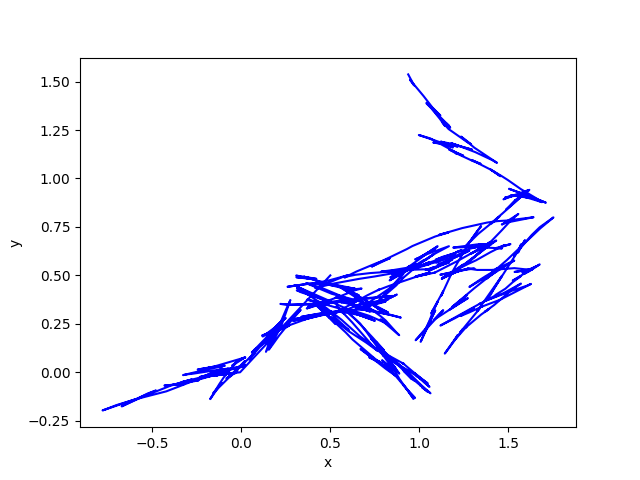
\includegraphics[width=90mm]{xy_coords_single_paths.png}
\end{center}
\end{frame}

\begin{frame}{Plot of a collection of random paths following $X,Y,$ in $(x,y,\theta)$ space}
\begin{center}
    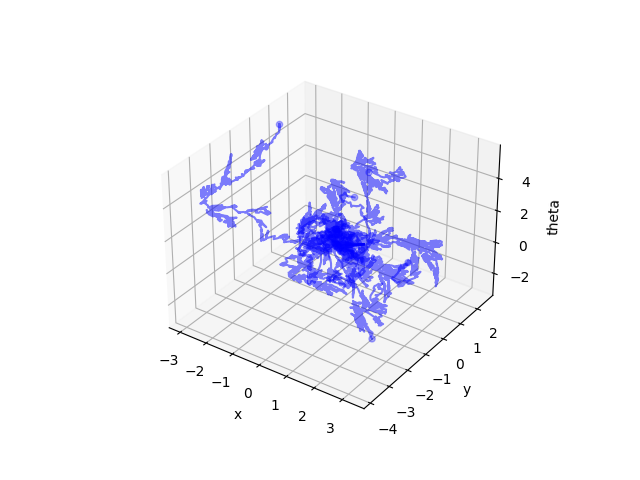
\includegraphics[width=100mm]{xyt_coords_multiple_paths.png}
\end{center}
\end{frame}

\begin{frame}{Another example: A rolling ball}
    Consider a ball rolling on a plane, without twisting or slipping:
    \begin{center}
    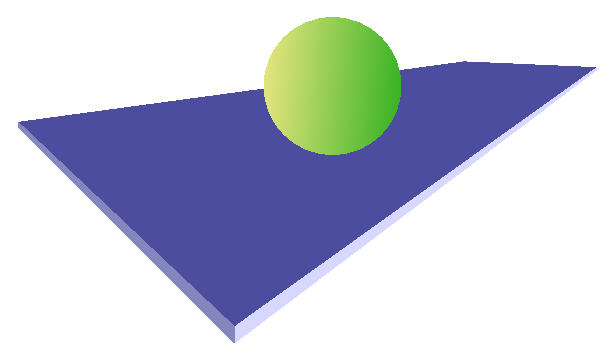
\includegraphics[width=100mm]{ballonplane.eps}
    \end{center}
\end{frame}

\begin{frame}{Rolling ball example (cont.)}
    The space of orientations of the ball is $M=\mathrm{SO}(3).$ The Lie algebra of $\mathrm{SO}(3)$ is spanned by three vector fields:
    \[
        X = \text{rolling around }x\text{ axis},\; Y = \text{ rolling around }y\text{ axis}
    \]
    and
    \[
        Z = \text{rolling around }z\text{ axis}.
    \]
    They satisfy $[X,Y]=Z,\, [Y,Z]=X$ and $[Z,X]=Y.$

    To say that the ball ``moves without twisting or slipping" is to say that the orientations of the ball move along the vector fields $X,Y.$
\pause
    Let
    \[
        H^1 = \mathrm{span}\{X,Y\}.
    \]
    Then
    \[
        0=H^1 < H^1 < H^2 = T\mathrm{SO}(3)
    \]
    is a Carnot structure for $\mathrm{SO}(3),$ and $X^2+Y^2$ is a hypoelliptic operator.
\end{frame}


\begin{frame}{Pseudodifferential operators on a Carnot manifold}
    Pseudodifferential operators on a manifold $M$ can normally be defined by
    \[
        Tu(x) = \int_{TM_x} K(x,z)u(\exp_x(z))\,dz,\quad u \in C^{\infty}(M)
    \]
    where $K$ is the kernel of a pseudodifferential operator on tangent space $TM_x.$ Something similar works for Carnot manifolds,
    \[
        Tu(x) = \int_{T_HM_x} K(x,z)u(\Lambda_x(z))\,dz
    \]
    where $K$ is the kernel of a pseudodifferential operator on the graded Lie group $T_HM_x,$ and $\Lambda$ is a very carefully chosen family of local diffeomorphisms.
\end{frame}

\begin{frame}{The right way to do it: The tangent groupoid}
    The main questions about defining pseudodifferential operators
    \[
        Tu(x) = \int_{T_HM_x} K(x,z)u(\Lambda_x(z))\,dz
    \]
    are:
    \begin{enumerate}[{\rm (i)}]
        \item{} What are the right conditions on the kernel function?
        \item{} What are the right conditions on the local diffeomorphisms $\Lambda_x$?
    \end{enumerate}
    These are quite tricky problems... several solutions exist (they are more-or-less equivalent).
\end{frame}

\begin{frame}{The right way to do it: The tangent groupoid}
    Van Erp and Yuncken proposed that the Schwartz kernels of pseudodifferential operators should be those which admit an approximately homogeneous
    extension to the $H$-tangent groupoid
    \[
        \Tb_HM := T_HM\times \{0\}\sqcup M\times M\times \Rl^{\times}
    \]
    (appropriately topologised).\\
    \pause
    The advantages of their approach is that it is manifestly coordinate invariant, and it makes some of the elementary $\psi$DO theory very easy.
\end{frame}



%
% \section{Analysis on singular foliations}\label{singular_section}
%
% \begin{frame}
%     \Huge{Section \ref{singular_section}: Analysis on singular foliations}\end{frame}
% \end{frame}
%
% \begin{frame}{The limitations of Carnot manifolds}
%     Not all H\"ormander sum of squares operators come from Carnot manifolds, some of them, like the Grushin operator
%     \[
%         G = -\partial_x^2-\sin^2(2\pi x)\partial_y
%     \]
%     come from so-called singular filtrations.
% \end{frame}
%
% \section{Weyl's law}\label{Weyl_section}
%
% \begin{frame}
%     \Huge{Part \ref{Weyl_section}: Weyl's law and hypoelliptic operators}
% \end{frame}
%
% \begin{frame}{Weyl's law for elliptic operators}
%     Let $P\geq 0$ be an elliptic pseudodifferential operator of order $m$ on a compact manifold $M,$ with principal symbol $\sigma_m.$ Weyl's law for elliptic operators says that asymptotically as $\lambda\to\infty,$ we have
%     \[
%         N(\lambda,P) \sim (2\pi)^{-d}|\{(x,\xi)\in T^*M\;:\;\sigma_m(x,\xi)\leq \lambda\}|
%     \]
%     where $|\cdot|$ is the phase-space volume (i.e. the Liouville measure).
%     Equivalently
%     \[
%         N(\lambda,P) \sim (2\pi)^{-d}\lambda^{\frac{d}{m}}|\{(x,\xi)\;:\;\sigma_m(P)(x,\xi)\leq 1\}|.
%     \]
% \end{frame}
%
% \begin{frame}{The Grushin puzzle}
%     Consider the following differential operator $G$ on the $2$-torus $\Circ^2 = \Rl^2/\Itgr^2,$
%     \[
%         G = -\partial_x^2-\sin^2(2\pi x)\partial_y^2,\quad \sigma_2(P)(x,\xi) = \xi_x^2+\sin^2(2\pi x)\xi_y^2.
%     \]
%     This is a so-called Grushin-type operator on the torus. It is not elliptic.\pause
%
%     Let $\Sigma(\lambda)$ be the region of phase space where the principal symbol of $G$ is $<\lambda,$ i.e.
%     \[
%         \Sigma(\lambda) := \{((x,y),(\xi_x,\xi_y))\in \Circ^2\times \Rl^2\;:\;\xi_x^2+\sin^2(2\pi x)\xi_y^2 \leq \lambda\}.
%     \]
%     This has infinite volume.
%     \[
%         |\Sigma(\lambda)| = \lambda\int_0^1 \frac{1}{|\sin(2\pi x)|}\,dx = +\infty.
%     \]
%     \pause
%     Nevertheless, $G$ has discrete spectrum, and there exists a constant $c$ such that
%     \[
%         N(\lambda,G) \sim c\lambda \log(\lambda),\quad \lambda\to\infty.
%     \]
%     (compare that an elliptic operator of order $2$ in dimension $2$ would have $N(\lambda)\sim c\lambda$).
%     What is going on here?
% \end{frame}
%
% \begin{frame}{Fefferman's interpretation}
%     In a famous paper titled ``the uncertainty principle", Fefferman gave a heuristic argument explaining why operators like $G$ have discrete spectrum and explaining the form of their spectral counting function.
%
%     The semiclassical heuristic suggests that
%     \[
%         N(\lambda,G)\sim \#\{\text{ states that can fit inside the region }\Sigma(\lambda)\}.
%     \]
%     By the uncertainty principle, a state should be localised in a region of volume at most $(2\pi)^d.$
% \end{frame}
%
% \begin{frame}{Fefferman's distorted boxes}
%     A \emph{distorted box} is a region in phase space of the form
%     \begin{align*}
%         \{(x,\xi)\;:\; |x-x_0|< \delta,\; |\xi-\xi_0|< \frac{1}{\delta}\}.
%     \end{align*}
%     Previously we estimated $N(\lambda,G)$ by the volume of $\Sigma(\lambda)$. Fefferman suggests to instead take:
%     \[
%         N(\lambda,G) \sim (2\pi)^{-d}\#\{\text{disjoint distorted boxes that can fit inside }\Sigma(\lambda)\}.
%     \]
%     It turns out that this right-hand-side is finite, and gives the correct asymptotic as $\lambda\to\infty.$
% \end{frame}
%


\section{Some recent results}\label{conclusion_section}

\begin{frame}
    \Huge{Part \ref{conclusion_section}: Conclusion and some results}
\end{frame}

\begin{frame}{Background on ideals}
    Let $H$ be a Hilbert space, and let $\Kc(H)$ denote the compact operators on $H.$
% The $n$th singular value $\mu(n,T)$ of $T \in \Kc(H)$ is defined as
%     \[
%         \mu(n,T) := \inf\{\|T-R\|_{\infty}\;:\;\mathrm{rank}(T)\leq n\}
%     \]
%     where $\|\cdot\|_{\infty}$ is the operator norm. Equivalently $\mu(n,T)=\lambda(n,|T|).$
    The trace ideal $\Lc_1$ is defined as
    \[
        \Lc_1(H) := \{T\in \Kc(H)\;:\;\|T\|_1 := \sum_{n=0}^\infty \lambda(n,|T|)\}
    \]
    and the weak-trace class ideal is defined as
    \[
        \Lc_{1,\infty}(H) := \{T \in \Kc(H)\;:\;\|T\|_{1,\infty} := \sup_{n\geq 0} (n+1)\lambda(n,|T|)\}.
    \]
\end{frame}

\begin{frame}{Background on traces}
    The trace ideal is so named because it's the natural domain of the operator trace
    \[
        \Tr:\Lc_1(H)\to \Cplx.
    \]
    In general, a trace on an operator ideal $\Ic$ is a unitarily invariant functional
    \[
        \varphi:\Ic\to \Cplx,\quad \varphi(UAU^*)=\varphi(A),\; \quad U \text{ unitary.}
    \]
    Equivalently $\varphi(AB)=\varphi(BA)$ for all $A \in \Ic$ and bounded $B.$
\end{frame}

\begin{frame}{The trace theorem}
    \begin{theorem}[Connes' trace theorem]\label{ctt_original}
        Let $M$ be a compact $d$-dimensional manifold and let $T\in \Psi^{-d}(M)$ be a classical pseudodifferential operator of order $-d.$ Let $\nu$ be a density on $M.$
        Then $T$ can be identified with an element of $\Lc_{1,\infty}(L_2(M,\nu))$ and for any normalised trace $\varphi$ on $\Lc_{1,\infty}(L_2(M,\nu))$ we have
        \[
            \varphi(T) = \frac{1}{d}\mathrm{Res}(T).
        \]
    \end{theorem}
\end{frame}

\begin{frame}{The trace theorem (without traces)}
    \begin{theorem}[Connes' trace theorem]\label{ctt_original}
        Let $M$ be a compact $d$-dimensional manifold and let $T\in \Psi^{-d}(M)$ be a classical pseudodifferential operator of order $-d.$ Let $\nu$ be a density on $M.$
        Then $T$ can be identified with an element of $\Lc_{1,\infty}(L_2(M,\nu))$ and for any normalised trace $\varphi$ on $\Lc_{1,\infty}(L_2(M,\nu))$ we have
        \[
            \sum_{n=0}^N \lambda(n,T) = \frac{1}{d}\mathrm{Res}(T)\log(N+2)+O(1),\quad N\to\infty..
        \]
    \end{theorem}
\end{frame}

\begin{frame}{Connes' trace theorem for Carnot manifolds}
    This is the obligatory part of the talk where I advertise my own results.
    \begin{theorem}
        Let $(M,H)$ be a compact Carnot manifold with homogeneous dimension $Q,$ and let $T \in \Psi^{-Q}_H(M)$ (in the van Erp--Yuncken sense). Then $T$ can be realised as an operator belonging to the weak-trace-class ideal $\Lc_{1,\infty},$ and for any normalised trace $\varphi$ on $\Lc_{1,\infty}$ we have
        \[
            \varphi(T) = \frac1Q\mathrm{Res}(T)
        \]
        where $\mathrm{Res}(T)$ is the residue as defined by Couchet--Yuncken.
    \end{theorem}
\end{frame}

\begin{frame}
\structure{\begin{center}
{\Huge{}Thank you for listening!}
\par\end{center}}
\end{frame}



\end{document}

